\documentclass[12pt,a4paper]{article}
\usepackage[utf8]{inputenc}
\usepackage[german]{babel}
\usepackage[T1]{fontenc}
\usepackage{amsmath}
\usepackage{amsfonts}
\usepackage{amssymb}
\usepackage{graphicx}
\usepackage[left=2cm,right=2cm,top=2cm,bottom=2cm]{geometry}
\author{Tim}

\begin{document}

\tableofcontents
\newpage

\section{Prismenspektrometer}

\subsection{Grundlagen}

\subsection{Dispersionskurve}
In diesem Teilversuch wurde die Dispersionskurve des verwendeten Prismas mithilfe einer Quecksilber-Cadmium-Lampe vermessen.

\subsection{Dispersionskurve}
In diesem Teilversuch wurde die Dispersionskurve des verwendeten Prismas mithilfe einer Quecksilber-Cadmium-Lampe vermessen.

\subsubsection{Aufbau und Durchführung}
Durch eine Kollimatorlinse werden ebene Wellenfronten erzeugt. Diese werden mit dem einem Drehteller befindlichen Prisma gebrochen. Das gebrochene Spaltbild wird mit einem schwenkbaren Fernrohr beobachtet. Die relative Position des Fernrohrs kann dabei auf 1' genau abgelesen werden.

In diesem Versuch werden zunächst die Minimalablenkungen des Prismas für mehrere Spektrallinien bestimmt.
Durch gleichsinniges Drehen von Prismenteller und Fernrohr wandern auch die Spektrallinien, zunächst in die eine und dann in die andere Richtung. Der Umkehrpunkt entspricht dabei der Minimalablenkung. Man wiederholt die Messung, diesmal trifft das Licht allerdings auf der anderen Prismenseite auf. Dann gilt für die Minimalablenkung

\begin{equation}
2 \delta_{min} = \psi_2-\psi_1
\end{equation}

wobei $\psi_i$ die Umkehrpunkte sind.
Zur Bestimmung der statistischen Unsicherheit auf die $\psi_i$ wurde eine Rauschmessung an der $\psi_1$-Position der blau-grünen Cadmiumlinie ($\lambda=508,58nm$) durchgeführt.

Für die übrigen Positionen der Spektrallinien wurde die Messung drei (bzw. fünf) mal wiederholt. Der Fehler auf die sich so ergebenden Mittelwert ist dann $\sigma_{\psi}=\frac{\sigma_{psi}}{\sqrt{N}}$.

Es ergeben sich damit die Minimalablenkungen und der Fehler auf selbige für jede vermessene Spektrallinie.

\begin{equation}
\sigma_{\delta} = \sqrt{\sigma_{\psi_1}^2+\sigma_{psi_2}^2}
\end{equation}

Damit folgt für die Brechungsindizes bei den entsprechenden Wellenlängen::

\begin{equation}
n = \frac{sin(\frac{\delta_{min}+\epsilon}{2})}{sin(\frac{\epsilon}{2})}
\end{equation}

\begin{equation}
\sigma_n = \frac{cos(\frac{\delta_{min}+\epsilon}{2})}{sin(\frac{\epsilon}{2})} \frac{\delta_{min}}{2}
\end{equation}

\subsubsection{Rohdaten}

\begin{table}
\begin{center}
\begin{tabular}{|c|c|}
\hline 
$\psi_1$ & $\psi_2$ \\ 
\hline 
25$^{\circ}$3' & 147$^{\circ}$21' \\ 
\hline 
25$^{\circ}$1' & 147$^{\circ}$22' \\ 
\hline 
25$^{\circ}$0'& 147$^{\circ}$13' \\ 
\hline 
25$^{\circ}$1' & 147$^{\circ}$11' \\ 
\hline 
25$^{\circ}$1' & 147$^{\circ}$16' \\ 
\hline 
25$^{\circ}$3' & \\ 
\hline 
25$^{\circ}$9' & \\ 
\hline 
25$^{\circ}$3' & \\ 
\hline 
25$^{\circ}$10' & \\ 
\hline 
25$^{\circ}$20' & \\ 
\hline 
25$^{\circ}$14' & \\ 
\hline 
25$^{\circ}$11' & \\ 
\hline 
25$^{\circ}$9' & \\ 
\hline 
25$^{\circ}$8' & \\ 
\hline 
25$^{\circ}$10' & \\ 
\hline 

\end{tabular} 
\label{tab:RauschenPrisma}
\caption{Rohdaten der grün-blauen Cadmiumlinie. Die Messwerte auf $\psi_1$ dienen als Rauschmessung für die statistische Unsicherheit .}
\end{center}
\end{table}


\begin{table}
\begin{center}
\begin{tabular}{|c|c|}
\hline
$\psi_1$ & $\psi_2$ \\
\hline
$\lambda =$404.66nm & \\
\hline
21$^{\circ}$2' &151$^{\circ}$15' \\
\hline
21$^{\circ}$0' &151$^{\circ}$14' \\
\hline
20$^{\circ}$56' &151$^{\circ}$18' \\ 
\hline
$\lambda =$435.83nm & \\
\hline
22$^{\circ}$43' &149$^{\circ}$34' \\
\hline
22$^{\circ}$45' &149$^{\circ}$33' \\ 
\hline
22$^{\circ}$42' &149$^{\circ}$33' \\ 
\hline
$\lambda =$467.81nm & \\
\hline
23$^{\circ}$55' &148$^{\circ}$22' \\
\hline
23$^{\circ}$54' &148$^{\circ}$24' \\
\hline
23$^{\circ}$57' &148$^{\circ}$20' \\ 
\hline
$\lambda =$479.99nm & \\
\hline
24$^{\circ}$22' &147$^{\circ}$56' \\ 
\hline
24$^{\circ}$24' &148$^{\circ}$0' \\ 
\hline
24$^{\circ}$18' &148$^{\circ}$2' \\ 
\hline
$\lambda =$564.07nm & \\
\hline
25$^{\circ}$53' &146$^{\circ}$24' \\
\hline
25$^{\circ}$54' &146$^{\circ}$25' \\
\hline
25$^{\circ}$54' &146$^{\circ}$22' \\ 
\hline
$\lambda =$579.07nm & \\
\hline
26$^{\circ}$34' &145$^{\circ}$48' \\
\hline
26$^{\circ}$32' &145$^{\circ}$44' \\
\hline
26$^{\circ}$33' &145$^{\circ}$44' \\ 
\hline
$\lambda =$643.85nm & \\
\hline
27$^{\circ}$20' &144$^{\circ}$57' \\
\hline
27$^{\circ}$20' &144$^{\circ}$55' \\
\hline
27$^{\circ}$24' &144$^{\circ}$59' \\
\hline
\end{tabular}
\label{tab:RohdatenDispersion}
\caption{Rohdaten für die Position der beiden Umkehrpunke für die vermessenen Spektrallinien der HgCa-Lampe. Die Wellenlängen sind dem Praktikumsskript (S.19) entnommen worden.}
\end{center}
\end{table}

Das Ergebnis der Rauschmessung zur Bestimmung des statistischen Fehlers für die Winkelmessung findet sich in Tabelle \ref{tab:RauschenPrisma}.
Die Rohdaten der restlichen Spektrallinien, welche Vermessen wurden sind in Tabelle \ref{tab:RohdatenDispersion} dargestellt.


\subsubsection{Auswertung}

\begin{table}
\begin{center}
\begin{tabular}{|c|c|c|}
\hline
$\lambda /nm$ & $\delta_{min} / rad$ & n \\
\hline
404.66 & 1.1368 $\pm$ 0.0007 & 1.7751$\pm$ 0.0004\\
\hline
435.83 & 1.1068$\pm$ 0.0007 & 1.7611$\pm$ 0.0004\\
\hline
467.81 & 1.086$\pm$ 0.0007 & 1.7511$\pm$ 0.0004\\
\hline
479.99 & 1.0789$\pm$ 0.0007&1.7477$\pm$ 0.0004\\
\hline
508.58 & 1.0661$\pm$ 0.0004 & 1.7414$\pm$ 0.0002\\
\hline
546.07 & 1.0516$\pm$ 0.0007 & 1.7342$\pm$ 0.0004\\
\hline
579.07 & 1.0403$\pm$ 0.0007 & 1.7286$\pm$ 0.0004\\
\hline
643.85 & 1.0262$\pm$ 0.0007 & 1.7215$\pm$ 0.0004\\
\hline
\end{tabular}
\label{tab:AuswertungDispersion}
\caption{Ergebnisse der Auswertung. Dargestellt ist der bestimmte minimale Ablenkungswinkel mit Unsicherheit für jede vermessene Linie sowie die sich daraus ergebenden Brechungsindizes.}
\end{center}
\end{table}

\begin{figure}
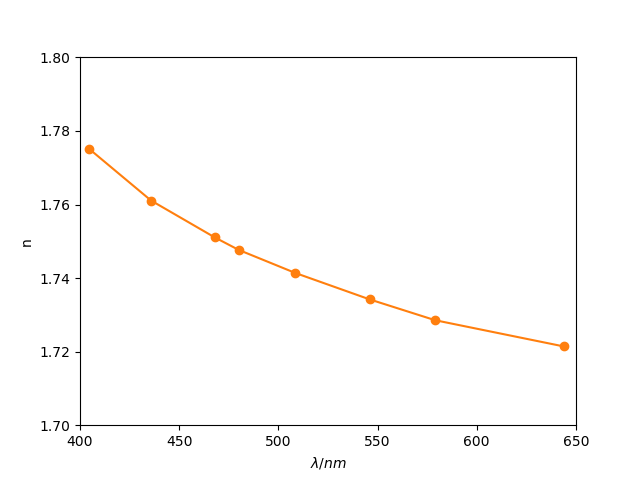
\includegraphics[scale=1.0]{Bilder/Dispersionskurve.png}
\label{fig:Dispersionskurve}
\caption{Die Dispersionskurve des verwendeten Prismas. Die Fehlerbalken auf die n-Werte sind relativ klein und somit nicht erkennbar. Die einzelnen Messpunkte wurden zur Veranschaulichung verbunden.}
\end{figure}

\begin{figure}
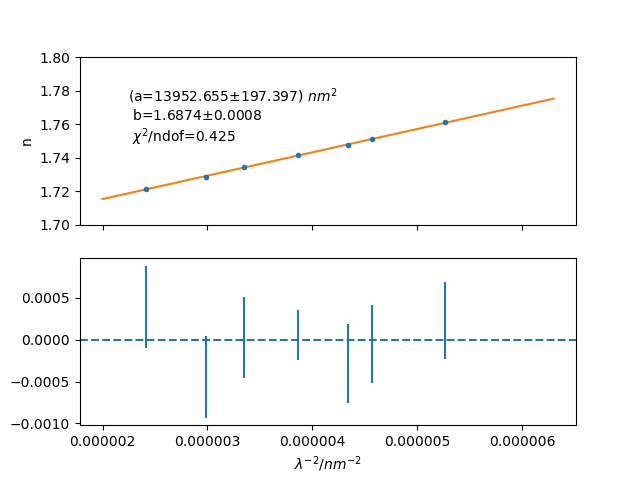
\includegraphics[scale=1.0]{Bilder/Regression.png}
\label{fig:RegressionDispersion}
\caption{Auftragung von n gegen $1/\lambda^2$. Das beste Anpassung ergab sich für eine Anpassungsgerade der Form $n(\lambda) = \frac{a}{\lambda^2} + b $}. Auch hier sind die Fehlerbalken aufgrund der geringen Größe kaum erkennbar.
\end{figure}


Die Rauschmessung ergibt eine statistische Unsicherheit auf die $\psi_i$ von $\sigma_{\psi_i} = 0.0017 rad$ bzw. $\sigma_{\psi_i} = 5.8'$. Wie in der Durchführung beschrieben kann nun aus den Daten die Minimalablenkung $\delta_{min}$ und der entsprechende Fehler, sowie aus diesen der Brechungsindex und seine Unsicherheit für die entsprechenden Wellenlängen berechnet werden.
Die Werte sind in Tabelle \ref{tab:AuswertungDispersion} dargestellt.

Durch Auftragen des Brechungsindex gegen die Wellenlänge erhält man die Dispersionskurve (Abb. \ref{fig:Dispersionskurve}).




\newpage
\section{Gitterspektrometer}

\subsection{Grundlagen}
\subsubsection{Beugung am Gitter}
Ein Gitter ist ein optisches Bauteil, das einfallendes Licht beugt. Das Beugungsmuster ist ähnlich dem der Beugung an einem Doppelspalt. Allerdings hat das Gitter gegenüber dem Doppelspalt einige Vorteile: Durch die hohe Anzahl der Spalte ist die durchgelassene Intensität deutlich höher als bei einem Doppelspalt. Zudem ermöglicht dies schmalere Spalte, welches eine besser Auflösung ermöglicht.\\
\begin{figure}
\begin{center}
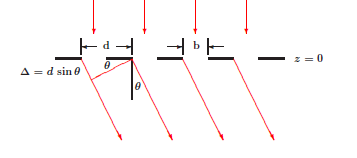
\includegraphics[scale=1.2]{Bilder/Gitterbeugung_Schema.PNG}
\end{center}
\caption[Gitterbeugung Schema]{Schematische Darstellung der Beugung an einem Gitter}
\label{fig:Gitterbeugung_Schema}
\end{figure}
Abbildung \ref{fig:Gitterbeugung_Schema} zeigt schematisch die Entstehung des Beugungsbildes durch den Gangunterschied zwischen zwei benachbarten Strahlen am Gitter. Wenn dieser Gangunterschied ein ganzzahliges Vielfaches der Wellenlänge ist, liegt konstruktive Interferenz vor und es ist ein Maximum zu sehen. Dies führt auf die wichtige Bedingung
\begin{equation}
d \sin (\theta) = n \lambda.
\label{eq:Maximumsbedingung}
\end{equation}
Dabei bezeichnet $n$ die Ordnung des Maximums. An dieser Beziehung lassen sich einige wichtige Bedingungen ablesen. Damit beobachtbare Beugung auftritt, muss $\lambda < d$ gelten. Die maximal beobachtbare Ordnung ist $n_{max} = \dfrac{d}{\lambda}$. \\
Wenn die Gitterebene nicht exakt senkrecht zum einfallenden Strahl steht, muss ein Gangunterschied zwischen den Strahlen vor dem Gitter berücksichtigt werden. Wenn $\varphi$ der Winkel zwischen der Senkrechten zum Lichtstrahl und der Gitterebene und $\theta$ der Beobachtungswinkel ist, kann Gl. \ref{eq:Maximumsbedingung} verallgemeinert werden zu:
\begin{equation}
d(\sin(\varphi) + \sin(\theta - \varphi)) = n \lambda
\label{eq:VerallgemeinerteMaximumsbedingung}
\end{equation}

\subsubsection{Auflösungsvermögen eines Gitters}
Für die Trennung zweier nah beieinander liegender Spektrallinien $\lambda$ und $\lambda + \Delta \lambda$ müssen nach dem Rayleigh-Kriterium das erste Beugungsmaximum der ersten Linie mit dem ersten Beugungsminimum der zweiten Linie zusammenfallen. Aus dieser Bedingung lässt sich für das Auflösungsvermögen eines Gitters die Beziehung
\begin{equation}
A \equiv \dfrac{\lambda}{\Delta \lambda} = n \cdot N
\label{eq:AuflösungsvermögenGitterspektrometer}
\end{equation}
herleiten. Dabei ist $n$ die Ordnung des betrachteten Maximums und $N$ die Zahl der beleuchteten Spalte des Gitters.

\subsection{Aufbau und Durchführung}
\begin{figure}
\begin{center}
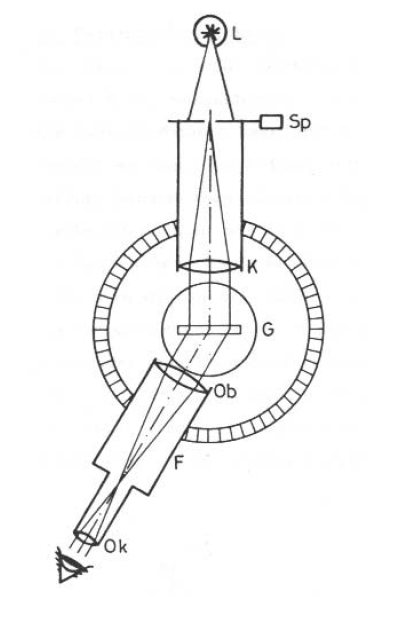
\includegraphics[scale=0.5]{Bilder/Schematischer_Aufbau_Gitterspektrometer.PNG}
\end{center}
\caption[Gitterspektrometer Aufbau Schema]{Schematische Darstellung des Versuchaufbaus der Beugung an einem Gitter}
\label{fig:Versuchsaufbau_Gitterbeugung_Schema}
\end{figure}
Abbildung \ref{fig:Versuchsaufbau_Gitterbeugung_Schema} zeigt schematisch den Aufbau eines Gitterspektrometers.\\
Eine Spektrallampe wird vor ein Kollimatorrohr gestellt. Dieses dient dazu, den Strahlengang möglichst parallel auf das Gitter zu schicken. An dem der Lampe zugewandten Ende des Kollimatorrohres ist ein in der Breite einstellbarer Spalt, der als zu beobachtender "Gegenstand" dient. Das Gitter steht auf einem Teller und wird dort (so gut wie möglich) senkrecht zum Kollimatorrohr aufgestellt. Sowohl das Gitter als auch das Kollimatorrohr werden einmal eingestellt und sollten danach nicht mehr bewegt werden. Bewegt wird nur das Fernrohr, mit dem die Beobachtung stattfindet. Dieses ist dazu auf einem drehbaren Arm angebracht, der mit einem Nonius verbunden ist, sodass ein Winkel abgelesen werden kann, mit dem dann die Beugung gemessen wird.\\
Zunächst muss ein Fehler auf die Winkelmessung bestimmt werden. Dazu wird die nullte Ordnung zehnmal gemessen. Um wirklich zehn einzelne, voneinander unabhängige Messungen zu erhalten, wird das Maximum jedes Mal komplett neu angefahren. Bei den nachfolgenden Messungen wird angenommen, dass der Fehler auf die Winkelmessung immer gleich ist und der Fehler aus der Rauschmessung übernommen. Da hierfür die Nullte Ordnung verwendet wird, kann der Mittelwert der Rauschmessung als Nullniveau verwendet werden. Die gemessenen Winkel müssen also immer als Abweichung von diesem Nullniveau betrachtet werden.\\
Für die Bestimmung der Gitterkonstanten eines (laut Herstellerangabe) sehr feinen Gitters muss eine Lampe mit vielen Spektrallinien im sichtbaren Bereich verwendet werden, da nach Gl. \ref{eq:Maximumsbedingung} nur wenige Ordnung beobachtbar sind. In diesem Fall wurde hierfür die Cadmium-Lampe verwendet. Es werden ausgewählte Spektrallinien in den beobachtbaren Ordnung angefahren und die Winkel gemessen. Wichtig ist, dass die Linien in Ordnung auf beiden Seiten der nullten Ordnung vermessen werden, um in der Anpassung berücksichtigen zu können, dass die Gitterebene nicht perfekt senkrecht zum einfallenden Strahl stand. Dabei werden die Ordnungen auf den beiden Seiten durch ein Vorzeichen unterschieden: Positives Vorzeichen bedeutet Drehung des Fernrohrs gegen den Uhrzeigersinn, negatives Vorzeichen Drehung im Uhrzeigersinn.\\
Zur Bestimmung der Wellenlänge der Spektrallinien einer anderen Lampe wird muss die Lampe ausgewechselt werden. Da hier eine Quecksilber-Cadmium Lampe verwendet wurde, muss darauf geachtet werden, dass nur die Quecksilber-Linien sinnvoll vermessen werden können. Die Durchführung ist identisch zu der Durchführung der Messung der Gitterkonstanten.\\
Zur Bestimmung des Auflösungsvermögens wird die Lampe durch eine andere ausgetauscht, die zwei nah beieinander liegende Spektrallinien hat. Hier wurden die beiden roten Linien der Natrium-Lampe verwendet. Es wird eine Leiste mit unterschiedlichen Blenden auf das Kollimatorrohr angebracht. Die Blenden haben Breiten in 0,5mm Schritten startend bei 0,5mm.\\
Die rote Doppellinie wird in erster Ordnung angefahren und in dem Okular so gelegt, dass sie gut sichtbar nicht zu weit am Rand liegt. Es ist darauf zu achten, dass das Fadenkreuz am Okular nicht die beiden Linien trennt. Anschließend wird in der Leiste der Blenden nach und nach eine kleinere Blende eingestellt und immer wieder überprüft, ob die beiden Linien noch getrennt werden können oder nicht.

\subsection{Bestimmung der Gitterkonstanten}

\subsection{Bestimmung der Wellenlänge}

\subsection{Bestimmung der Auflösung}

\subsection{Zusammenfassung}


\end{document}